\subsection{Walled Game}

When the arena is walled off and the agents are not able to fall off of the board, it is hypothesized that the prey will Figure out some sort of move pattern to avoid the predator quickly, and the predator should be able to quickly adapt to the prey and capture it. This would show on fitness graphs as lines representing the predators and prey crossing over each other as they keep adapting to capture or escape respectively. This type of behaviour is not seen in any of the walled off game graphs, although the fitnesses do fluctuate in tandem with each other, just not as extremely as expected. Furthermore, the prey always outperforms the predator in the walled off game. The general pattern of all of the graphs tends to be a sharp improvement in the beginning of the run, and then the curve flattens out as seen in Figure \ref{fig:wall-exp-1} which both came from the same experiment. In most cases the fitness of the particles at the end of the run are determined by the gain/loss that occurred at the beginning of the run. A more promising run that seems like it would have improved if training time was longer can be seen in Figure \ref{fig:walled-better-run}. 

\begin{figure}
  \centering
  \begin{subfigure}{0.7\textwidth}
  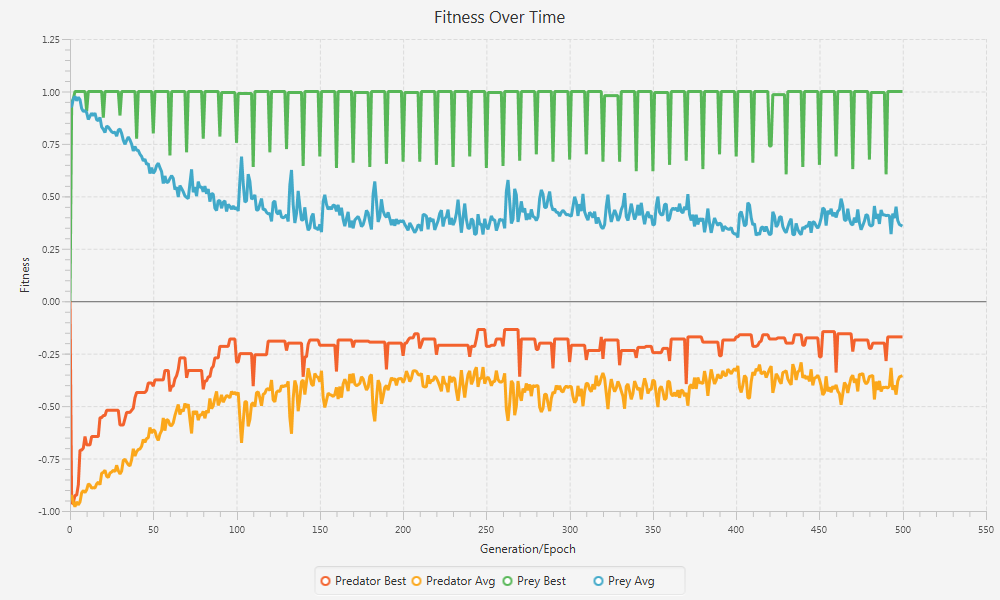
\includegraphics[width=\linewidth]{V3-false-rc5-pl30-pdh0-pdc30-pyh0-pyc30-r0.png}
  \caption{Run 0}
  \end{subfigure}
  \begin{subfigure}{0.7\textwidth}
    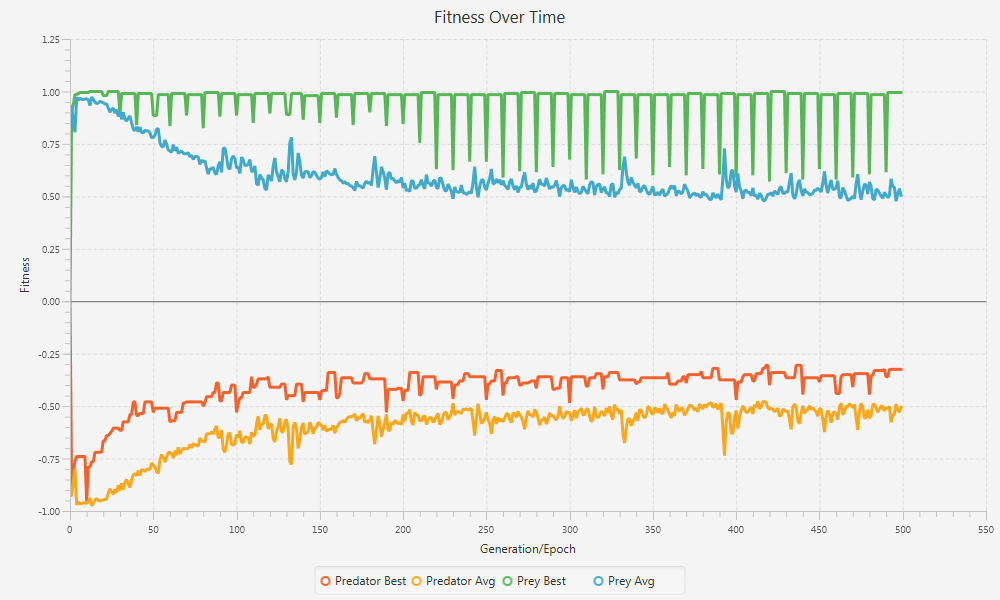
\includegraphics[width=\linewidth]{V3-false-rc5-pl30-pdh0-pdc30-pyh0-pyc30-r2.png}
    \caption{Run 2}
    \end{subfigure}
  \caption{Experiment 13 fitness over time}
  \label{fig:wall-exp-1}
\end{figure}

\begin{figure}
  
   \centering
  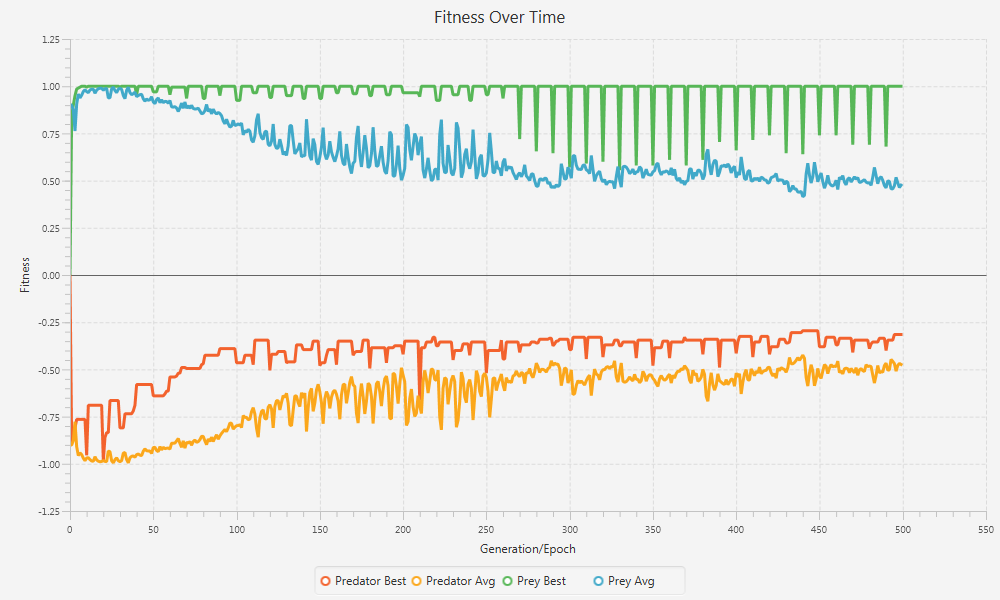
\includegraphics[width=0.7\textwidth]{V3-false-rc2-pl40-pdh0-pdc15-pyh0-pyc15-r3.png}  
  \caption{Experiment 1 run 2 fitness over time}
  \label{fig:walled-better-run}
  
\end{figure}

In the walled game, although the overall population performance for the predator is not great, there tends to be at least one strong particle that is much higher than the rest of the swarm. This can be seen in Figures \ref{fig:walled-good-1} and \ref{fig:walled-good-2}. An example of the types of games this type of particle plays can be seen in Figure \ref{fig:walled-good-game-ex}. In this case, the prey always seems to want to leave the stage. However, since it cannot, it seems to get stuck, and then the predator just approaches and captures the prey. Although this is a very simple scenario, the path of the predator is quite direct when going to capture the prey, as such it demonstrates that the predator is capable of learning to capture the prey.


\begin{figure}
  \centering
  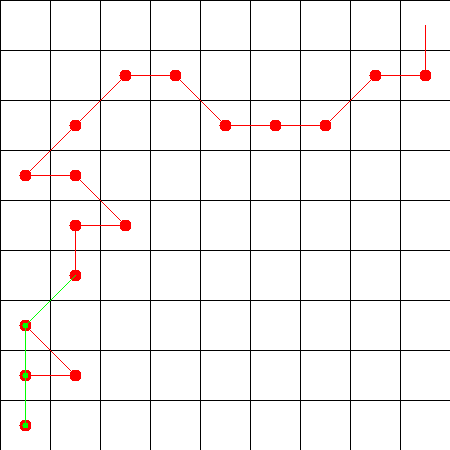
\includegraphics[width=0.4\textwidth]{walled-good-ex-1.png}   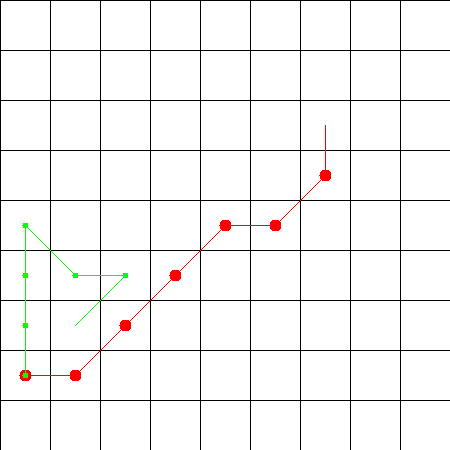
\includegraphics[width=0.4\textwidth]{walled-good-ex-2.png}
  \caption{Experiment 15 run 2:  Example games}
  \label{fig:walled-good-game-ex}
\end{figure}

\begin{figure}
   \centering
  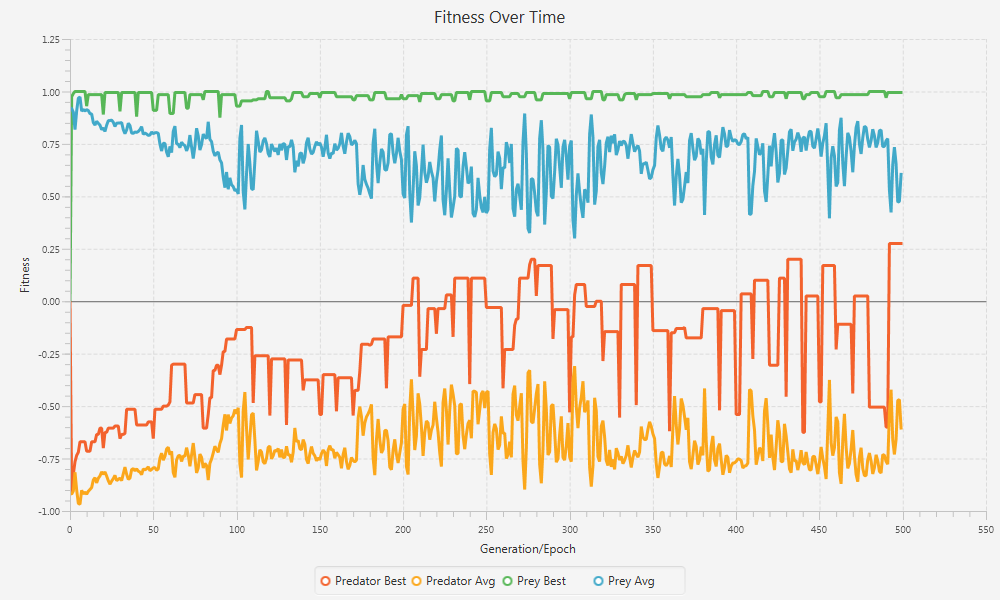
\includegraphics[width=0.7\textwidth]{V3-false-rc5-pl30-pdh067-pdc30-pyh067-pyc30-r2.png}  
  \caption{Experiment 15 run 2 fitness over time}
  \label{fig:walled-good-1}
\end{figure}


\begin{figure}
   \centering
  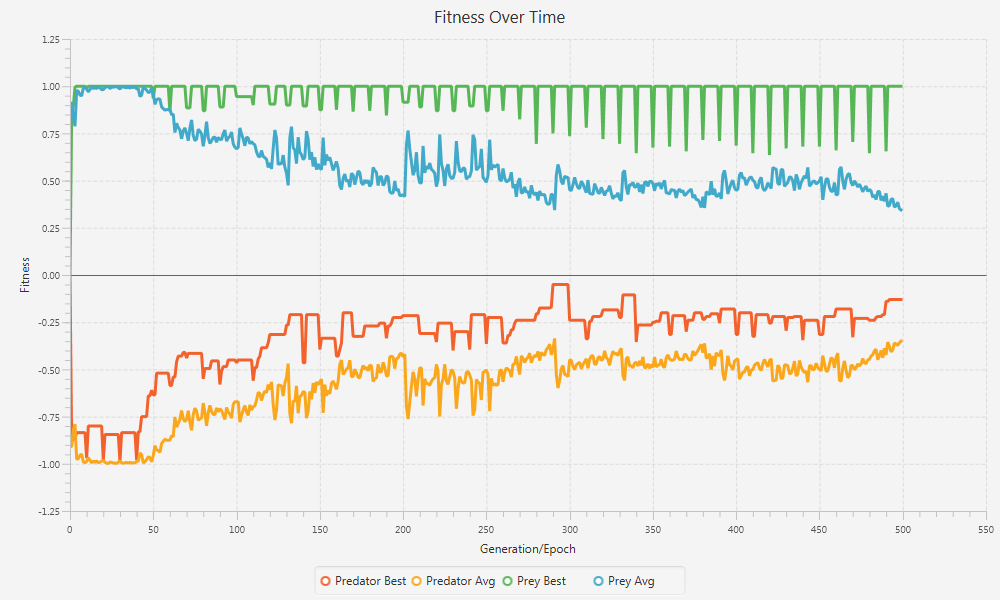
\includegraphics[width=0.7\textwidth]{V3-false-rc5-pl30-pdh033-pdc15-pyh033-pyc15-r1.png}  
  \caption{Experiment 6 run 1 fitness over time}
  \label{fig:walled-good-2}
\end{figure}


\begin{table}
  \centering
  \begin{tabular}{|c|c|c|c|c|c|c|}
    \hline
    \multirow{2}{*}{Experiment} & \multicolumn{3}{|c|}{Predator} & \multicolumn{3}{|c|}{Prey} \\\cline{2-7}
    & Max & Average & Min & Max & Average & Min\\
    \hline
    1 & -0.235 & -0.363 & -0.475 & 0.995 & 0.964 & 0.943 \\
2 & 0.065 & -0.245 & -0.455 & 0.980 & 0.965 & 0.942 \\
3 & -0.055 & -0.278 & -0.465 & 0.994 & 0.973 & 0.940 \\
4 & -0.125 & -0.271 & -0.460 & 0.988 & 0.969 & 0.939 \\
5 & -0.200 & -0.312 & -0.405 & 0.997 & 0.960 & 0.918 \\
6 & -0.050 & -0.253 & -0.450 & 0.999 & 0.993 & 0.984 \\
7 & -0.075 & -0.291 & -0.440 & 0.981 & 0.953 & 0.922 \\
8 & 0.025 & -0.160 & -0.415 & 0.992 & 0.973 & 0.944 \\
9 & -0.135 & -0.284 & -0.415 & 0.984 & 0.974 & 0.964 \\
10 & -0.305 & -0.392 & -0.430 & 0.995 & 0.963 & 0.914 \\
11 & -0.125 & -0.307 & -0.430 & 0.991 & 0.966 & 0.911 \\
12 & -0.230 & -0.309 & -0.340 & 0.989 & 0.969 & 0.937 \\
13 & -0.135 & -0.355 & -0.500 & 0.977 & 0.961 & 0.933 \\
14 & -0.145 & -0.355 & -0.505 & 0.967 & 0.955 & 0.937 \\
15 & 0.275 & -0.131 & -0.370 & 0.985 & 0.974 & 0.957 \\
16 & -0.195 & -0.310 & -0.385 & 0.994 & 0.980 & 0.957 \\
17 & -0.260 & -0.358 & -0.540 & 0.996 & 0.979 & 0.966 \\
18 & -0.285 & -0.392 & -0.445 & 0.998 & 0.963 & 0.926 \\
19 & 0.015 & -0.213 & -0.430 & 0.988 & 0.979 & 0.968 \\
20 & -0.195 & -0.343 & -0.465 & 0.988 & 0.947 & 0.918 \\
21 & -0.040 & -0.297 & -0.420 & 0.988 & 0.960 & 0.946 \\
22 & -0.125 & -0.273 & -0.440 & 0.994 & 0.973 & 0.943 \\
23 & 0.005 & -0.296 & -0.555 & 0.993 & 0.969 & 0.939 \\
24 & -0.040 & -0.330 & -0.455 & 0.994 & 0.961 & 0.921 \\

    \hline
  \end{tabular}
  \caption{Walled Game Summary}
  \label{tab:walled-summary}
\end{table}